\documentclass[11pt, a4paper]{report}
\usepackage[utf8]{inputenc}
\usepackage{lscape}   % Make a page in landscape format \begin{landscape}
\usepackage{colortbl} % To color table cells
\usepackage{color} % Able to change textcolor
\usepackage[table]{xcolor}
\usepackage{longtable}
\usepackage{graphicx} % Able to add pictures
\usepackage{parskip}  % Separate paragraphs with a blank line
                      % rather than using indentation
\usepackage{hyperref} % Support for hyperlinks
\usepackage[protrusion=true,expansion=true]{microtype} % Improve justification
\usepackage{subfigure}
\usepackage{hyperref}
\usepackage{caption}
\usepackage{float}
\usepackage{afterpage}
\usepackage{lipsum}
\usepackage{wrapfig}
\usepackage{array}
\usepackage{sidecap}
\usepackage{appendix}
\usepackage{fancyhdr}
\usepackage{changepage}
\usepackage{tabularx}
\usepackage{multirow}


\hypersetup{%
    pdfborder = {0 0 0}
}

\begin{document}
	\begin{titlepage}
\begin{center}

{\Huge \bf Compendium} \\[1.0cm]
{\Huge \bf TDT4237 - Software Security}\\[1.0cm]
{\Large \bf Part Two} \\

{\Large OWASP Testing Guide}

\vspace{14cm}

\centering
{\Large \bf By Marte Løge}



\end{center}
\end{titlepage}
	\clearpage
	\tableofcontents

	\clearpage

	\chapter{Introduction to Security Testing}
	\clearpage
	\section{The OWASP Testing Guide}
		{\bf OWASP:} The Open Web Application Security Project

		The OWASP Testing Project has been in development for many years. With this project, 
		we wanted to help people understand the what, why, when, where, and how of testing their 
		web applications, and not just provide a simple checklist or prescription of issues 
		that should be addressed. The outcome of this project is a complete Testing Framework, 
		from which others can build their own testing programs or qualify other people’s 
		processes. The Testing Guide describes in details both the general Testing Framework and 
		the techniques required to implement the framework in practice.

		\section{What, Why, When?}

		{\bf What is Testing?} \\
		What do we mean by testing? During the development life cycle of a web application, 
		many things need to be tested. The Merriam-Webster Dictionary describes testing as:
			\begin{itemize}
				\item To put to test or proof.
				\item To undergo a test.
				\item To be assigned a standing or evaluation based on tests.
			\end{itemize}
		Many outsiders regard security testing as a black art. This document’s aim is to
		change that perception and to make it easier for people without in-depth security 
		knowledge to make a difference.

		{\bf Why Testing?} \\
		This document is designed to help organizations understand what comprises a testing 
		program, and to help them identify the steps that they need to undertake to build 
		and operate that testing program on their web applications. 
		It is intended to give a broad view of the elements required to make a comprehensive 
		web application security program. 
		This guide can be used as a reference and as a methodology to help determine the gap 
		between your existing practices and industry best practices. 
		This guide allows organizations to compare themselves against industry peers, understand 
		the magnitude of resources required to test and maintain their software, or prepare for 
		an audit. 
		The technical details about how to test an application, as part of a penetration test or code review, will be covered in later chapters. 

		\clearpage
		{\bf When to Test?} \\ 
		Most people today don’t test the software until it has already been created and is in 
		the deployment phase of its life cycle (i.e., code has been created and instantiated 
		into a working web application). 
		This is generally a very ineffective and cost-prohibitive practice. One of the best 
		methods to prevent security bugs from appearing in production applications is to 
		improve the Software Development Life Cycle (SDLC) by including security in each of 
		its phases. 

		An SDLC is a structure imposed on the development of software artifacts. If an SDLC 
		is not currently being used in your environment, it is time to pick one! 
		The following figure shows a generic SDLC model: 

		\begin{figure} [H]
			\centering
			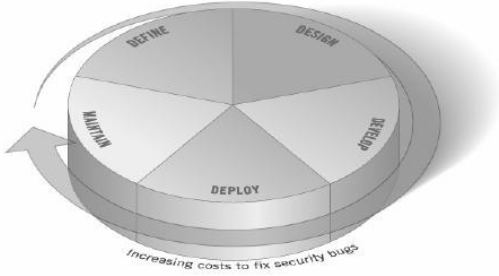
\includegraphics[scale=0.5]{pics/SDCL.png}
		\end{figure}


		{\bf What to Test?} \\
		It can be helpful to think of software development as a combination of people, process, 
		and technology. If these are the factors that "create" software, then it is logical 
		that these are the factors that must be tested. Today most people generally
		test the technology or the software itself. An effective testing program should 
		have components that test \\
		{\bf People} – to ensure that there is adequate education and
		awareness; \\ 
		{\bf Process} – to ensure that there are adequate policies and standards and 
		that people know how to follow these policies; \\ 
		{\bf Technology} – to ensure that the process has been effective in its implementation. 

		\clearpage
		\section{Principles of Testing}

			{\bf There is no silver bullet: } While it is tempting to think that a security 
			scanner or application firewall will either provide a multitude of defenses or
			identify a multitude of problems, in reality there are no silver bullets to the 
			problem of insecure software.

			{\bf Think strategically, not tactically: } The patch-and-penetrate model involves
			fixing a reported bug, but without proper investigation of the root cause. 
			This model is usually associated with the window of vulnerability:

				\begin{figure}[H]
					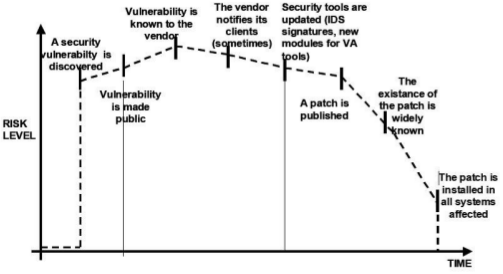
\includegraphics[scale=0.7]{pics/windowOfExposure.png}
				\end{figure}


			To prevent reoccurring security problems within an application, it is essential 
			to build security into the Software Development Life Cycle (SDLC) by developing
			standards, policies, and guidelines that fit and work within the development
			methodology. Threat modeling and other techniques should be used to help assign
			appropriate resources to those parts of a system that are most at risk.


			{\bf Test early and test often: } When a bug is detected early within the SDLC, 
			it can be addressed more quickly and at a lower cost. A security bug is no
			different from a functional or performance-based bug in this regard.


			{\bf Understand the scope of security:} It is important to know how much security 
			a given project will require. The information and assets that are to be protected
			should be given a classification that states how they are to be handled (e.g., Confidential, Secret, Top Secret). Security testing cost money! You have to
			prioritize what's important for your system. 

			\clearpage
			{\bf Develop the right mindset: } Successfully testing an application for security
			vulnerabilities requires thinking "outside of the box." Normal use cases will
			test the normal behavior of the application when a user is using it in the manner 
			that you expect. Good security testing requires going beyond what is expected and
			thinking like an attacker who is trying to break the application. This is one of 
			the reasons why automated tools are actually bad at automatically testing for
			vulnerabilities.

			{\bf Understand the subject: } One of the first major initiatives in any good 
			security program should be to require accurate documentation of the application. 
			The architecture, data-flow diagrams, use cases, and more should be written in 
			formal documents and made available for review. 

			{\bf Use the right tools: } While we have already stated that there is no silver 
			bullet tool. There is a range of open source and commercial tools that can 
			automate many routine security tasks. These tools can simplify and speed up the 
			security process. It is important to understand exactly what these tools can 
			and cannot do.

			{\bf The devil is in the details: } It is critical not to perform a superficial
			security review of an application and consider it complete. Care should be taken 
			to verify that every possible section of application logic has been tested, and 
			that every use case scenario was explored for possible vulnerabilities.

			{\bf Use source code when available: } While black box penetration test results 
			can be impressive and useful to demonstrate how vulnerabilities are exposed in
			production, they are not the most effective way to secure an application. 
			If the source code for the application is available, it should be given to the 
			security staff to assist them while performing their review. 
			It is possible to discover vulnerabilities within the application source that 
			would be missed during a black box engagement.

			{\bf Develop metrices: } An important part of a good security program is the 
			ability to determine if things are getting better. It is important to track
			the results of testing engagements, and develop metrics that will reveal the
			application security trends within the organization. 

			{\bf Document the test results: } To conclude the testing process, it is 
			important to produce a formal record of what testing actions were taken, 
			by whom, when they ware performed, and details of the test findings.


	\clearpage
	\section{Testing Techniques}

		This section presents a high-level overview of various testing techniques that 
		can be employed when building a testing program.

		\subsection{Manual Inspection and Reviews}
			Manual inspections are human-driven reviews that typically test the security
			implications of the people, policies, and processes, but can include inspection 
			of technology decisions such as architectural designs.
			By asking someone how something works and why it was implemented in a specific way, 
			it allows the tester to quickly determine if any security concerns are likely to 
			be evident. Manual inspections and reviews are one of the few ways to test
			the software development life-cycle process itself and to ensure that there is 
			an adequate policy or skill set in place. 
			As with many things in life, when conducting manual inspections and reviews we suggest you adopt a trust-but-verify model. 

			{\bf Advantages:}
			\begin{itemize}
				\item Requires no supporting technology
				\item Can be applied to a variety of situations
				\item Flexible
				\item Promotes teamwork
				\item Can be performed early in the SDLC
			\end{itemize}

			{\bf Disadvantages:}
			\begin{itemize}
				\item Can be time consuming
				\item Supporting material not always available
				\item Requires significant human thought and skill to be effective!
			\end{itemize}

		\clearpage
		\subsection{Threat Modeling}
			Threat modeling has become a popular technique to help system designers think 
			about the security threats that their systems/applications might face. 
			Therefore, threat modeling can be seen as risk assessment for applications. 
			In fact, it enables the designer to develop mitigation strategies for potential
			vulnerabilities and helps them focus their inevitably limited resources and 
			attention on the parts of the system that most require it.
			To develop a threat model, we recommend taking a simple approach.
			This approach involves:

			\begin{itemize}
				\item {\bf Defining and classifying the assets} – classify the assets into tangible and intangible assets and rank them according to business importance.
				\item {\bf Exploring potential vulnerabilities} - whether technical, operational, 
				or management.
				\item {\bf Decomposing the application} – how the application works, its assets,
				functionality, and connectivity.
				\item {\bf Exploring potential threats} – use threat scenarios and/or attack trees.
				\item {\bf Creating mitigation strategies} – develop mitigating controls for each of the threats deemed to be realistic.
			\end{itemize}

			{\bf Advantages:}
				\begin{itemize}
					\item Practical attacker's view of the system
					\item Flexible
					\item Early in the SDLC
				\end{itemize}

			{\bf Disadvantages:}
				\begin{itemize}
					\item Relatively new technique
					\item Good threat models don’t automatically mean good software
				\end{itemize}

		\clearpage
		\subsection{Source Code Review}
			Source code review is the process of manually checking a web application's source 
			code for security issues. Many serious security vulnerabilities cannot be detected 
			with any other form of analysis or testing. As the popular saying goes “if you
			want to know what’s really going on, go straight to the source." Almost all 
			security experts agree that there is no substitute for actually looking at the 
			code. All the information for identifying security problems is there in the code
			somewhere.

			{\bf Advantages:}
			\begin{itemize}
				\item Completeness and effectiveness
				\item Accuracy
				\item Fast (for competent reviewers)
			\end{itemize}
			{\bf Disadvantages:}
			\begin{itemize}
				\item Requires highly skilled security developers
				\item Can miss issues in compiled libraries
				\item Cannot detect run-time errors easily
				\item The source code actually deployed might differ from the one being analyzed
			\end{itemize}

		\clearpage	
		\subsection{Penetration Testing}

		Penetration testing has been a common technique used to test network security for 
		many years. It is also commonly known as black box testing or ethical hacking. 
		Penetration testing is essentially the “art” of testing a running application remotely,
		without knowing the inner workings of the application itself, to find security
		vulnerabilities. Typically, the penetration test team would have access to an 
		application as if they were users. The tester acts like an attacker and attempts 
		to find and exploit vulnerabilities. 
		Penetration testing tools have been developed that automate the
		process, but, again, with the nature of web applications their effectiveness is 
		usually poor. 

		Gary McGraw summed up penetration testing well when he said: \\
		{\bf “If you fail asummed penetration test you know you have a very bad problem indeed. 
		If you pass a penetration test you do not know that you don’t have a very bad problem”.}

		{\bf Advantages:}
		\begin{itemize}
			\item Can be fast (and therefore cheap)
			\item Requires a relatively lower skill-set than source code review
			\item Tests the code that is actually being exposed
		\end{itemize}

		{\bf Disadvantages:}
		\begin{itemize}
			\item Too late in the SDLC
			\item Front impact testing only!
		\end{itemize}

		\clearpage
		\subsection{Test Effort According to Test Technique}
			With so many techniques and so many approaches to testing the security of web
			applications, it can be difficult to understand which techniques to use and when 
			to use them. The fact remains that all techniques should probably be used to 
			ensure that all areas that need to be tested are tested. What is clear, however, 
			is that there is no single technique that effectively covers all security testing 
			that must be performed to ensure that all issues have been addressed. The following
			figure shows a typical proportional representation of test effort according to 
			test technique:

			\begin{figure}[H]
				\centering
				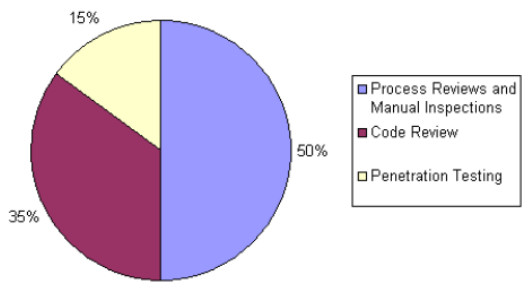
\includegraphics[scale=0.6]{pics/effort.png}
			\end{figure}

	\clearpage
	\section{Security Requirements}

		\subsection{Test Derivation}

		{\bf Testing Objectives} \\
		One of the objectives of security testing is to validate that security controls function as 
		expected. This is documented via {\bf security requirements} that describe the functionality 
		of the security control. At a high level, this means proving confidentiality, integrity, and 
		availability of the data as well as the service. The other objective is to validate that security
		controls are implemented with few or no vulnerabilities. These are common vulnerabilities, 
		such as the OWASP Top Ten, as well as vulnerabilities that are previously identified with 
		security assessments during the SDLC, such as threat modeling, source code analysis, and 
		penetration test. \\

		{\bf Security Requirement Documentation} \\
		The first step in the documentation of security requirements is to understand the 
		business requirements. A {\bf business requirement document} could provide the initial, 
		high-level information of the expected functionality for the application. For example, 
		the main purpose of an application may be to provide financial services to customers or 
		shopping and purchasing goods from an on-line catalogue. A security section of the business 
		requirements should highlight the need to protect the customer data as well as to comply 
		with applicable security documentation such as regulations, standards, and policies.

		Applicable {\bf industry standards} for security need also to be captured by the general security 
		requirement checklist. For example, in the case of applications that handle customer credit 
		card data, the compliance with the PCI DSS standard forbids the storage of PINs and CVV2 data.

		Another section of the checklist needs to enforce general requirements for compliance with the 
		{\bf organization information security standards and policies}. From the functional requirements 
		perspective, requirement for the security control needs to map to a specific section of the 
		information security standards. An example of such requirement can be: {\bf "a password
		complexity of six alphanumeric characters must be enforced by the authentication controls 
		used by the application."} \\

		{\bf Security Requirements Validation} \\
		From the functionality perspective, the validation of security requirements is the main objective of 
		security testing, while, from the risk management perspective, this is the objective of information 
		security assessments. More in depth, the security assessment objective is risk analysis, such
		as the identification of potential weaknesses in security controls that ensure the confidentiality, 
		integrity, and availability of the data. 
		Assuming encryption is used to protect the data, encryption algorithms and key
		lengths need to comply with the {\bf organization encryption standards}. For example, a security 
		requirement that can be security tested is verifying that only allowed ciphers are used 
		(e.g., SHA-1, RSA, 3DES) with allowed minimum key lengths (e.g., more than 128 bit for symmetric 
		and more than 1024 for asymmetric encryption).

		From the security assessment perspective, security requirements can be validated at different 
		phases of the SDLC by {\bf using different artifacts and testing methodologies}. For example, threat 
		modeling focuses on identifying security flaws during design, secure code analysis and reviews 
		focus on identifying security issues in source code during development, and penetration testing 
		focuses on identifying vulnerabilities in the application during testing/validation.

		{\bf Threats and Countermeasures Taxonomies}\\
		A {\bf threat and countermeasure classification} that takes into consideration root causes of 
		vulnerabilities is the critical factor to verify that security controls are designed, coded, 
		and built so that the impact due to the exposure of such vulnerabilities is mitigated.

		The focus of a threat and countermeasure {\bf categorization} is to define security requirements 
		in terms of the threats and the root cause of the vulnerability. The root cause can be 
		categorized as security flaw in design, a security bug in coding, or an issue due to insecure 
		configuration. 	A threat and countermeasure categorization for vulnerabilities can also be used to 
		document security requirements for secure coding such as secure coding standards. An example of 
		a common coding error in authentication controls consists of applying an hash function to encrypt a 
		password, without applying a seed to the value. 


		{\bf Security Testing and Risk Analysis}\\
		By combining the results of source code analysis and penetration testing it is possible to determine 
		the likelihood and exposure of the vulnerability and calculate the risk rating of the vulnerability. 
		For example, high and medium risk vulnerabilities can be prioritized for remediation, while low risk 
		can be fixed in further releases.
		By considering the threat scenarios exploiting common vulnerabilities it is possible to identify 
		potential risks for which the application security control needs to be security tested. By thinking 
		in terms of threats and vulnerabilities, it is possible to devise a battery of tests that simulate 
		such attack scenarios.


		\subsection{Positive Requirements}
			From the perspective of functional security requirements, the applicable standards, policies 
			and regulations drive both the need of a type of security control as well as the control  
			functionality. These requirements are also referred to as {\bf “positive requirements”}, 
			since they state the expected functionality that can be validated through security tests. 
			Examples of positive requirements are: 
				\begin{itemize}
					\item The application will lockout the user after six failed logon attempts.
					\item Passwords need to be six min characters, alphanumeric.
				\end{itemize}
			The validation of positive requirements consists of asserting the expected functionality and, 
			as such, can be tested by re-creating the testing conditions, and by running the test according 
			to predefined inputs and by asserting the expected outcome as a fail/pass condition.
			In order to validate security requirements with security tests, security requirements need to 
			be function driven and highlight the expected functionality {\bf (the what)} and implicitly 
			the implementation {\bf (the how)}. Examples of high-level security design requirements for 
			authentication can be:

				\begin{itemize}
					\item Protect user credentials and shared secrets in transit and in storage
					\item Mask any confidential data in display (e.g., passwords, accounts)
					\item Lock the user account after a certain number of failed login attempts
					\item Do not show specific validation errors to the user as a result of failed logon
					\item Only allow passwords that are alphanumeric, include special characters and six 
				\end{itemize}

		\subsection{Negative Requirements}
			Security tests need also to be risk driven, that is they need to validate the application for 
			unexpected behavior. These are also called {\bf “negative requirements”}, since they specify 
			what the application should not do. Examples of "should not do" (negative) requirements are:
				\begin{itemize}
					\item The application should not allow for the data to be altered or destroyed
					\item The application should not be compromised or misused for unauthorized financial 
					transactions by a malicious user.
				\end{itemize}

			Negative requirements are more difficult to test, because there is no expected behavior to look for. 
			This might require a threat analyst to come up with unforeseeable input conditions, causes, and 
			effects. This is where security testing needs to be driven by risk analysis and threat modeling. 
			The key is to document the threat scenarios and the functionality of the countermeasure as a factor 
			to mitigate a threat. For example, in case of authentication controls, the following security
			requirements can be documented from the threats and countermeasure perspective:

				\begin{itemize}
					\item Encrypt authentication data in storage and transit to mitigate risk of information
					disclosure and authentication protocol attacks.
					\item Encrypt passwords using non reversible encryption such as using a digest (e.g., HASH) 
					and a seed to prevent dictionary attacks.
					\item Lock out accounts after reaching a logon failure threshold and enforce password 
					complexity to mitigate risk of brute force password attacks
					\item Display generic error messages upon validation of credentials to mitigate risk 
					of account harvesting/enumeration.
				\end{itemize}

			Threat modeling artifacts such as {\bf threat trees and attack libraries} can be useful to derive the 
			negative test scenarios. A threat tree will assume {\bf a root attack} and identify different
			{\bf exploits of security controls} and necessary {\bf countermeasures} that could be validated to 
			be effective in mitigating such attacks.

		\subsection{Use and Misuse Cases}
			Pre-requisite in describing the application functionality is to understand what the application 
			is supposed to do and how. This can be done by describing use cases. {\bf Use cases}, in the 
			graphical form as commonly used in software engineering, show the interactions of actors and 
			their relations, and help to identify the actors in the application, their relationships, the
			intended sequence of actions for each scenario, alternative actions, special requirements, 
			and pre- and post-conditions.

			Similar to use cases, {\bf misuse and abuse cases} describe unintended and malicious use scenarios 
			of the application. These misuse cases provide a way to describe scenarios of how an attacker 
			could misuse and abuse the application. By going through the individual steps in a use scenario 
			and thinking about how it can be maliciously exploited, potential flaws or aspects of the application 
			that are not well-defined can be discovered. The key is to describe all possible or, at least, the
			most critical use and misuse scenarios. Misuse scenarios allow the analysis of the application from 
			the {\bf attacker's point of view}.

			\clearpage
			{\bf Sequrity Requirements Derivation Through Use and Misuse Cases:}
				\begin{itemize}
					\item Step 1: Describe the Functional Scenario: 
					\item Step 2: Describe the Negative Scenario: 
					\item Step 3: Describe Functional and Negative Scenarios With Use and Misuse Case:
					\item Step 4: Elicit The Security Requirements. These security requirements need to be 
					documented and tested.

				\end{itemize}

			\begin{figure}[H]
				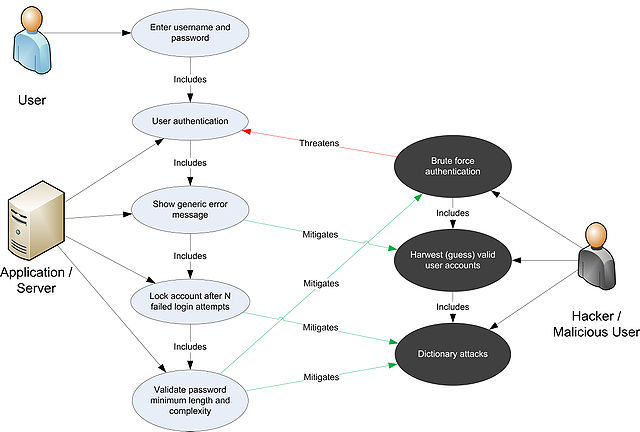
\includegraphics[width=\textwidth]{pics/useAndMisuse.jpg}
			\end{figure}
	\clearpage
	\section{Security Tests Integrated in Developers and Testers Workflow}

		\subsection{ Developers' Security Testing Workflow}
			Security testing during the development phase of the SDLC represents the first 
			opportunity for developers to ensure that individual software components that they 
			have developed are security tested before they are integrated with other components 
			and built into the application. Software components might consist of software artifacts 
			such as functions, methods, and classes, as well as application programming interfaces, 
			libraries, and executables. For security testing, developers can rely on the results of 
			{\bf the source code analysis} to verify statically that the developed source code does 
			not include potential vulnerabilities and is compliant with the secure coding standards. 
			{\bf Security unit tests} can further verify dynamically (i.e., at run time) that the 
			components function as expected.
		\subsection{Testers' Security Testing Workflow}
			After components and code changes are tested by developers and checked in to the application 
			build, the most likely next step in the software development process workflow is to perform 
			tests on the application as a whole entity. This level of testing is usually referred to as 
			{\bf integrated test} and {\bf system level test}. 
			These security tests on the application include both {\bf white box testing}, such as source 
			code analysis, and {\bf black box testing}, such as penetration testing. {\bf Gray box testing} 
			is similar to Black box testing. In a gray box testing we can assume we have some partial 
			knowledge about the session management of our application, and that should help us in 
			understanding whether the logout and timeout functions are properly secured.
			A testing engineer who validates the security of the application in the integrated system 
			environment might release the application for testing in the operational environment 
			(e.g., {\bf user acceptance tests}). The application {\bf functional testing} is usually 
			a responsibility of {\bf QA testers}, while {\bf white-hat hackers/security consultants} 
			are usually responsible for {\bf security testing}. 

	\clearpage
	\section{Security Test Data Analysis And Reporting}

	\subsection{Goals for Security Test Metrices and Measurements}
		The definition of the goals for the security testing metrics and measurements is a pre-requisite 
		for using security testing data for risk analysis and management processes. For example, a 
		measurement such as the {\bf total number of vulnerabilities found} with security tests might quantify 
		the security posture of the application. These measurements also help to identify security 
		objectives for software security testing: for example, reducing the number of vulnerabilities to 
		an acceptable number (minimum) before the application is deployed into production.

		From the perspective of the {\bf effort required to fix} a defect, both security and quality defects 
		can be measured in terms of developer hours to implement the fix, the tools and resources required 
		to fix, and, finally, the cost to implement the fix.

		Security testing data needs to support the security risk strategy at critical checkpoints during 
		the SDLC. For example, vulnerabilities found in source code with source code analysis represent 
		an initial measure of risk. Such {\bf measure of risk (e.g., high, medium, low)} for the vulnerability 
		can be calculated by determining the exposure and likelihood factors and, further, by validating 
		such vulnerability with penetration tests. The risk metrics associated to vulnerabilities found 
		with security tests empower business management to make {\bf risk management decisions}, such as to 
		decide whether risks can be accepted, mitigated, or transferred at different levels within the 
		organization.

		We need to lowering the cost of fixing the vulnerabilities, since it is less expensive to deal with the 
		vulnerabilities when they are found (in the same phase of the SDLC), rather than fixing them 
		later in another phase.

		When security test data is reported it has to provide metrics to support the analysis. The scope 
		of the analysis is the interpretation of test data to find clues about the security of the software 
		being produced as well the effectiveness of the process. Some examples of clues supported by security 
		test data can be:

		Are vulnerabilities reduced to an acceptable level for release? Are all security test requirements being met?
		What are the major root causes of security issues? Which security activity is most effective in finding vulnerabilities? Which team is more productive in fixing security defects and vulnerabilities? 
		Which percentage of overall vulnerabilities are high risks? Which tools are most effective in detecting security vulnerabilities?

		\subsection{Reporting Requirements}

			The security posture of an application can be characterized from the perspective of the effect, 
			such as number of vulnerabilities and the risk rating of the vulnerabilities, as well as from 
			the perspective of the cause (i.e., origin) such as coding errors, architectural flaws, and 
			configuration issues.

			When reporting security test data, the best practice is to include the following information, 
			besides the categorization of each vulnerability by type:
				\begin{itemize}
					\item The security threat that the issue is exposed to
					\item The root cause of security issues (e.g., security bugs, security flaw)
					\item The testing technique used to find it
					\item The remediation of the vulnerability (e.g., the countermeasure)
					\item The risk rating of the vulnerability (High, Medium, Low)
				\end{itemize}

		\subsection{Business Cases}
			For the security test metrics to be useful, they need to {\bf provide value} back to the organization's 
			security test data stakeholders, such as project managers, developers, information security offices,
			auditors, and chief information officers. The value can be in terms of the business case that each 
			project stakeholder has in terms of role and responsibility.

			{\bf Project managers} look for data that allows them to successfully manage and utilize security testing
			activities and resources according to the project plan. 

			To compliance {\bf auditors}, security test metrics provide a level of software security assurance and
			confidence that security standard compliance is addressed through the security review processes 
			within the organization.

			Finally, {\bf Chief Information Officers (CIOs) and Chief Information Security Officers (CISOs)}, 
			responsible for the budget that needs to be allocated in security resources, look for derivation 
			of a {\bf cost/benefit analysis} from security test data to make informed decisions on which security 
			activities and tools to invest. 












	\clearpage
	\chapter{Testing Framework}
	\clearpage
	\chapter{Web Application Penetration Testing}

	\section{Introduction to Penetration Testing}

	\subsection*{What is Web Application Penetration Testing?}

		A penetration test is a method of evaluating the security of a computer system or network 
		by simulating an attack. A Web Application Penetration Test focuses only on evaluating the 
		security of a web application. The process involves an active analysis of the application 
		for any weaknesses, technical flaws, or vulnerabilities. 

	\subsection*{What is a vulnerability?}
		{\bf A vulnerability} is a flaw or weakness in a system's design, implementation, or operation 
		and management that could be exploited to violate the system's security policy. 
		
		{\bf A threat} is a potential attack that, by exploiting a vulnerability, may harm the assets 
		owned by an application (resources of value, such as the data in a database or in the file system). 

		{\bf A test} is an action that tends to show a vulnerability in the application.

	\subsection*{What is the OWASP testing methodology?}
		{\bf Penetration testing} will never be an exact science where a complete list of all possible 
		issues that should be tested can be defined. Indeed, penetration testing is only an appropriate
		technique for testing the security of web applications under certain circumstances. 

		{\bf The goal} is to collect all the possible testing techniques, explain them and keep the 
		guide updated. The OWASP Web Application Penetration Testing method is based on the {\bf black box}
		approach. The tester knows nothing or very little information about the application to be tested. 

		{\bf The testing model consists of:}
			\begin{itemize}
				\item {\bf Tester:} Who performs the testing activities
				\item {\bf Tools and methodology:} The core of this Testing Guide project
				\item {\bf Application:} The black box to test
			\end{itemize}

	\subsection*{Active and Passive Mode}

		{\bf Passive Mode:} in the passive mode, the tester tries to understand the application's logic, 
		and plays with the application. Tools can be used for information gathering, for example, an 
		HTTP proxy to observe all the HTTP requests and responses. At the end of this phase, the tester 
		should understand all the access points (gates) of the application (e.g., HTTP headers, parameters,
		and cookies). The Information Gathering section explains how to perform a passive mode test.

		{\bf Ative Mode:}  in this phase, the tester begins to test (the penetration testing) using 
		the methodology described in the specific penetration category.

	\section{Overview Of Penetration Testing}

		\begin{tabularx}{15cm}{| X | X | X | X |}	
			\hline
			\rowcolor[gray]{.9}
			{\bf Category} &  {\bf Ref. Number} & {\bf Test Name} & {\bf Vulnerability} \\ \hline
			\multirow{6}{*}{\begin{minipage}{0.7in} Information Gathering \end{minipage}} & 
			OWASP-IG-001 & Spiders, Robots and Crawlers & 
			N.A. \\ \cline{2-4}
			 & OWASP-IG-002 & Search Engine Discovery & N.A \\ \cline{2-4}
			 & OWASP-IG-003 & Identify application entry points & N.A \\ \cline{2-4}
		 	 & OWASP-IG-004 & Testing for Web Application Fingerprints & N.A \\ \cline{2-4}
			 & OWASP-IG-005 & Application Discovery & N.A \\ \cline{2-4}
			 & OWASP-IG-006 & Analysis of Error Codes & Information Disclosure \\ \hline
		\end{tabularx}

		\begin{tabularx}{15cm}{| X | X | X | X |}	
			\hline
			\rowcolor[gray]{.9}
			{\bf Category} &  {\bf Ref. Number} & {\bf Test Name} & {\bf Vulnerability} \\ \hline
			\multirow{8}{*}{\begin{minipage}{0.7in} Configuration Management Testing \end{minipage}} & 
			OWASP-CM-001 & SSL/TLS Testing (SSL Version, Algorithms, Key length, Digital Cert. Validity) & 
			SSL Weakness \\ \cline{2-4}
			 & OWASP-CM-002 & DB Listener Testing & DB Listener weak \\ \cline{2-4}
			 & OWASP-CM-003 &  Infrastructure Configuration Management Testing & Infrastructure 
			 Configuration  management weakness \\ \cline{2-4}
		 	 & OWASP-CM-004 & Application Configuration Management Testing  &  Application
		 	 Configuration management weakness \\ \cline{2-4}
			 & OWASP-CM-005 &  &  \\ \cline{2-4}
			 & OWASP-CM-006 &  &  \\ \cline{2-4}
			 & OWASP-CM-007 &  &  \\ \cline{2-4}
			 & OWASP-CM-008 &  &  \\ \hline
		\end{tabularx}
	\clearpage
	\chapter{Information Gathering}
	\clearpage
	\chapter{Configuration Management Testing}
	Often analysis of the infrastructure and topology architecture can reveal a great deal about a 
	web application. Information such as source code, HTTP methods permitted, administrative 
	functionality, authentication methods and infrastructural configurations can be obtained.

\clearpage
\section{SSL/TLS Testing}
	The http clear-text protocol is normally secured via an SSL or TLS tunnel, resulting in 
	https traffic. In addition to providing encryption of data in transit, https allows the 
	identification of servers (and, optionally, of clients) by means of digital certificates.

	In order to detect possible support of weak ciphers, the ports associated to SSL/TLS wrapped 
	services must be identified. These typically include port 443 which is the standard https port, 
	however this may change because a) https services may be configured to run on non-standard ports, 
	and b) there may be additional SSL/TLS wrapped services related to the web 
	application. In general a service discovery is required to identify such ports. Vulnerability 
	Scanners, in addition to performing service discovery, may include checks against weak ciphers.

	\begin{figure}[H]
		\centering
		
\includegraphics{pics/ssl.jpg}
	\end{figure}

\section{DB Listener Testing}
	The Data base listener is a network daemon. It waits for connection requests from remote
	clients. This daemon can be compromised and hence can affect the availability of the database.

	It listens for connection requests and handles them accordingly. The listener, by default, 
	listens on port 1521(different ports may be used depending on the configuration). It is
	good practice to change the listener from this port to another arbitrary port number. 
	If this listener is "turned off" remote access to the database is not possible. If this 
	is the case, one’s application would fail also creating a denial of service attack.

	Potential areas of attack
	\begin{itemize}
		\item Stop the Listener -- create a DoS attack.
		\item Set a password and prevent others from controlling the Listener - Hijack the DB.
		\item Write trace and log files to any file accessible to the process owner of tnslnsr 
		- Possible informationleakage.
		\item Obtain detailed information on the Listener, database, and application configuration.
	\end{itemize}



\section{Infrastructure Configuration Management Testing}
	Proper configuration management of the web server infrastructure is very important in order 
	to preserve the security of the application itself. If elements such as the web server 
	software, the back-end database servers, or the authentication servers are not properly reviewed 
	and secured, they might introduce undesired risks or introduce new vulnerabilities that might
	compromise the application itself.

	In order to test the configuration management infrastructure, the following steps need to be taken:
		\begin{itemize}
			\item The different elements that make up the infrastructure need to be determined in 
			order to understand how they interact with a web application and how they affect 
			its security.
			\item All the elements of the infrastructure need to be reviewed in order to make sure 
			that they don’t hold any known vulnerabilities.
			\item A review needs to be made of the administrative tools used to maintain all the 
			different elements.
			\item The authentication systems, if any, need to reviewed in order to assure that 
			they serve the needs of the application and that they cannot be manipulated by external 
			users to leverage access.
			\item A list of defined ports which are required for the application should be maintained 
			and kept under change control.
		\end{itemize}


\section{Application Configuration Management Testing}
	Proper configuration of the single elements that make up an application architecture is important 
	in order to prevent mistakes that might compromise the security of the whole architecture.

	{\bf Sample/known files and directories}\\
	Many web servers and application servers provide, in a default installation, sample applications 
	and files that are provided for the benefit of the developer and in order to test that the server 
	is working properly right after installation. However, many default web server applications have 
	been later known to be vulnerable.

	{\bf Comment review} \\
	It is very common, and even recommended, for programmers to include detailed comments on their 
	source code in order to allow for other programmers to better understand why a given decision 
	was taken in coding a given function. Programmers usually do it too when developing large 
	web-based applications. However, comments included inline in HTML code might reveal to a 
	potential attacker internal information that should not be available to them. Sometimes, even
	source code is commented out since a functionality is no longer required, but this comment is 
	leaked out to the HTML pages returned to the users unintentionally. Comment review should be 
	done in order to determine if any information is being leaked through comments.

	{\bf Configuration review}
	The web server or application server configuration takes an important role in protecting the 
	contents of the site and it must be carefully reviewed in order to spot common configuration 
	mistakes. Obviously, the recommended configuration varies depending on the site policy, 
	and the functionality that should be provided by the server software. In most cases, however,
	configuration guidelines (either provided by the software vendor or external parties) should 
	be followed in order to determine if the server has been properly secured. It is impossible 
	to generically say how a server should be configured, however, some common guidelines should 
	be taken into account:

		\begin{itemize}
			\item Only enable server modules that are needed for the application. This reduces 
			the attack surface since the server is reduced in size and complexity as software 
			modules are disabled.
			\item Handle server errors with custom-made pages instead of with the default web 
			server pages. Specifically make sure that any application errors will not be returned 
			to the end-user and that no code is leaked through these since it will help an attacker. 
			\item Make sure that the server software runs with minimised privileges in the operating 
			system. 
			\item Make sure the server software logs properly both legitimate access and errors.
			\item Make sure that the server is configured to properly handle overloads and prevent 
			Denial of Service attacks. Ensure that the server has been performance tuned properly.
		\end{itemize}

	{\bf Logging} \\
	Logging is an important asset of the security of an application architecture, since it can be used 
	to detect flaws in applications as well as sustained attacks from rogue users. 
	In both cases (server and application logs) several issues should be tested and analysed based on 
	the log contents:
		\begin{itemize}
			\item Are the logs stored in a dedicated server?
			\item Can log usage generate a Denial of Service condition?
			\item How are they rotated? Are logs kept for the sufficient time?
			\item Do the logs contain sensitive information?
			\item How are logs reviewed? Can administrators use these reviews to detect 
			targeted attacks?
			\item How are log backups preserved?
			\item Is the data being logged data validated (min/max length, chars etc) 
			prior to being logged?
		\end{itemize}

\section{Testing for File Extensions Handling}
	File extensions are commonly used in web servers to easily determine which technologies 
	/ languages / plugins must be used to fulfill the web request.

	Determining how web servers handle requests corresponding to files having different extensions 
	may help to understand web server behaviour depending on the kind of files we try to access. 
	For example, it can help understand which file extensions are returned as text/plain versus 
	those which cause execution on the server side. The latter are indicative of technologies / 
	languages / plugins which are used by web servers or application servers, and may provide 
	additional insight on how the web application is engineered. For example, a “.pl” extension 
	is usually associated with server-side Perl support.

	The following file extensions should NEVER be returned by a web server, since they are related 
	to files which may contain sensitive information, or to files for which there is no reason to 
	be served.
		\begin{itemize}
			\item .asa
			\item .inc
		\end{itemize}

	The following file extensions are related to files which, when accessed, are either displayed 
	or downloaded by the browser. Therefore, files with these extensions must be checked to verify 
	that they are indeed supposed to be served (and are not leftovers), and that they do not contain
	sensitive information.
		\begin{itemize}
			\item {\bf .java:} No reason to provide access to Java source files
			\item {\bf .txt:} Text files
			\item {\bf .zip, .tar, .gz, .tgz, .rar, ...:} (Compressed) archive files
			\item {\bf .pdf:} PDF documents
			\item {\bf .doc, .rtf, .xls, .ppt, ...:} Office documents
			\item {\bf .bak, .old} and other extensions indicative of backup files 
			(for example: ~ for Emacs backup files)
		\end{itemize}

\section{Old, Backup and Unreferenced Files}

	While most of the files within a web server are directly handled by the server itself it 
	isn't uncommon to find {\bf unreferenced and/or forgotten files} that can be used to obtain 
	important information about either the infrastructure or the credentials. Most common 
	scenarios include the presence of renamed old version of modified files, inclusion files 
	that are loaded into the language of choice and can be downloaded as source, or even 
	automatic or manual backups in form of compressed archives.

	An important source of vulnerability lies in {\bf files which have nothing to do with the 
	application}, but are created as a consequence of editing application files, or after 
	creating on-the-fly backup copies, or by leaving in the web tree old files or unreferenced 
	files. Performing in-place editing or other administrative actions on production web servers 
	may inadvertently leave, as a consequence, backup copies.

	As a result, these activities generate files which 
	a) are not needed by the application, 
	b) may be handled differently than the original file by the web server. 

	For example, {\bf if we make a copy of login.asp named login.asp.old}, we are allowing users to
	download the source code of login.asp; this is because, due to its extension, login.asp.old 
	will be typically served as text/plain, rather than being executed. In other words, accessing 
	login.asp causes the execution of the server-side code of login.asp, while accessing 
	login.asp.old causes the content of login.asp.old (which is, again, server-side code) to be 
	plainly returned to the user – and displayed in the browser. This may pose security risks, 
	since sensitive information may be revealed. Generally, exposing server side code is a bad 
	idea; not only are you unnecessarily exposing business logic, but you
	may be unknowingly revealing application-related information which may help an attacker, 
	not to mention the fact that there are too many scripts with embedded username/password 
	in clear text (which is a careless and very dangerous practice).

	Other causes of unreferenced files are due to design or configuration choices when they 
	allow diverse kind of application- related files such as data files, configuration files, 
	log files, to be {\bf stored in filesystem directories} that can be accessed by the
	web server. These files have normally no reason to be in a filesystem space which could 
	be accessed via web, since they should be accessed only at the application level, by the 
	application itself (and not by the casual user browsing around!).

	{\bf Countermeasures}
	To guarantee an effective protection strategy, testing should be compounded by a security 
	policy which clearly forbids dangerous practices, such as:

		\begin{itemize}
			\item Editing files in-place on the web server / application server filesystem. 
			This is a particular bad habit, since it is likely to unwillingly generate backup 
			files by the editors. It is amazing to see how often this is done, even in large
			organizations.
			\item Check carefully any other activity performed on filesystems exposed by the 
			web server, such as spot administration activities. For example, if you occasionally 
			need to take a snapshot of a couple of directories (which you shouldn’t, on a 
			production system...), you may be tempted to zip/tar them first. Be careful not to 
			forget behind those archive files!
			\item Appropriate configuration management policies should help not to leave around 
			obsolete and unreferenced files.
			\item Applications should be designed not to create (or rely on) files stored under 
			the web directory trees served by the web server. Data files, log files, configuration 
			files, etc. should be stored in directories not accessible by the web server, to 
			counter the possibility of information disclosure
		\end{itemize}


\section{Infrastructure and Application Admin Interfaces}

	Administrator interfaces may be present in the application or on the application server to allow 
	certain users to undertake privileged activities on the site. Tests should be undertaken to 
	reveal if and how this privileged functionality can be accessed by an unauthorized or standard 
	user. An application may require an administrator interface to enable a privileged user to access
	functionality that may make changes to how the site functions. Such changes may include:
		\begin{itemize}
			\item User account provisioning
			\item Site design and layout
			\item Data manipultion
			\item Configuration changes
		\end{itemize}

	In many instances, such interfaces are usually implemented with little thought of how to separate 
	them from the normal users of the site. 

\section{Testing for HTTP Methods and XST}
	HTTP offers a number of methods that can be used to perform actions on the web server. Many of 
	theses methods are designed to aid developers in deploying and testing HTTP applications. 
	These HTTP methods can be used for nefarious purposes if the web server is misconfigured. 
	Additionally, Cross Site Tracing (XST), a form of cross site scripting using the servers 
	HTTP TRACE method, is examined.

	the Hypertext Transfer Protocol (HTTP) allows several other methods. 
	Here are the following eight methods: {\bf GET, POST, PUT, DELETE, TRACE, HEAD, 
	OPTIONS and CONNECT}

	Some of these methods can potentially pose a security risk for a web application, as they allow 
	an attacker to modify the files stored on the web server and, in some scenarios, steal the 
	credentials of legitimate users. More specifically, the methods that should be disabled are 
	the following:
		\begin{itemize}
			\item {\bf PUT:} This method allows a client to upload new files on the web server. 
			\item {\bf DELETE:} This method allows a client to delete a file on the web server. 
			\item {\bf CONNECT:} This method could allow a client to use the web server as a proxy
			\item {\bf TRACE:} This method simply echoes back to the client whatever string has been sent 
			to the server, and is used mainly for debugging purposes.
		\end{itemize}
		
	\clearpage
	\chapter{Authentication Testing}

	Authentication is the act of establishing or confirming something (or someone) as authentic, 
	that is, that claims made by or about the thing are true. Authenticating an object may
	mean confirming its provenance, whereas authenticating a person often consists of verifying her 
	identity. Authentication depends upon one or more authentication factors. In computer security,
	authentication is the process of attempting to verify the digital identity of the sender of a
	communication. A common example of such a process is the logon process. Testing the authentication 
	schema means understanding how the authentication process works and using that information to 
	circumvent the authentication mechanism.

\clearpage

\section{Credentials Transport Over An Encrypted Channel}
	Testing for credentials transport means to verify that the user's authentication data are transferred 
	via an encrypted channel to avoid being intercepted by malicious users. The analysis focuses simply 
	on trying to understand if the data travels unencrypted from the web browser to the server, or if the 
	web application takes the appropriate security measures using a protocol like HTTPS. The HTTPS protocol 
	is built on TLS/SSL to encrypt the data that is transmitted and to ensure that user is being sent towards
	the desired site. Clearly, the fact that traffic is encrypted does not necessarily mean that it's
	completely safe. The security also depends on the encryption algorithm used and the robustness of the 
	keys that the application is using, but this particular topic will not be addressed in this section. 

	Nowadays, the most common example of this issue is the login page of a web application. In order to 
	log into a web site, usually, the user has to fill a simple form that transmits the inserted data with 
	the POST method. What is less obvious is that this data can be passed using the HTTP protocol, that 
	means in a non-secure way, or using HTTPS, which encrypts the data.

	It is strongly suggested to use the POST method instead og GET. This is because when the GET method 
	is used, the url that it requests is easily available from, for example, the server logs exposing 
	your sensitive data to information leakage.

		\begin{figure}[H]
			
\includegraphics[scale=0.4]{pics/https.jpg}
		\end{figure}

\section{User Enumeration}

	The scope of this test is to verify if it is possible to collect a set of valid usernames by 
	nteracting with the authentication mechanism of the application. This test will be useful for the 
	brute force testing, in which we verify if, given a valid username, it is possible to find the
	corresponding password. Often, web applications reveal when a username exists on system, either 
	as a consequence of a misconfiguration or as a design decision. For example, sometimes, when we 
	submit wrong credentials, we receive a message that states that either the username is present 
	on the system or the provided password is wrong. 

	In some cases, we receive a message that reveals if the provided credentials are wrong because an 
	invalid username or an invalid password was used. Sometimes, we can enumerate the existing users 
	by sending a username and an empty password.

	{\bf Testing for nonexisting username} \\
	Generally the application should respond with the same error message and length to the different 
	wrong requests. If you notice that the responses are not the same, you should investigate and find 
	out the key that creates a difference between the 2 responses. For example:

	{\color{red} Client request: Valid user/wrong password -- Server answer:'The password is not correct'}

	{\color{red} Client request: Wrong user/wrong password -- Server answer:'User not recognized'}

	{\bf URI Probing} \\
	Sometimes a web server responds differently if it receives a request for an existing directory or 
	not. For instance in some portals every user is associated with a directory, if we try to access 
	an existing directory we could receive a web server error. A very common error that we can receive 
	from web server is:

	\begin{itemize}
		\item {\bf 403 Forbidden error code}
		\item {\bf 404 Not found error code}
		\item http://www.foo.com/account1 - we receive from web server: 403 Forbidden
		\item http://www.foo.com/account2 - we receive from web server: 404 file Not Found
	\end{itemize}

	In first case the user exists, but we cannot view the web page, in second case instead the user
	“account2” doesn’t exist. Collecting this information we can enumerate the users.

	{\bf Guessing Users} \\
	In some cases the userIDs are created with specific policies of administrator or company. 
	Other possibilities are userIDs associated with credit card numbers, or in general a numbers 
	with a pattern. For example we can view a user with a userID created in sequential order:

	{\color{blue} CN000100, CN000101, .....}

\section{Guessable User Account}

	Today's web applications typically run on popular open source or commercial software that is 
	installed on servers and requires configuration or customization by the server administrator. 
	In addition, most of today's hardware appliances, i.e., network routers and database servers, 
	offer web-based configuration or administrative interfaces.

	In addition, it is typical to find generic accounts, left over from testing or administration,
	that use common usernames and passwords and are left enabled in the application and its 
	infrastructure. These default username and password combinations are widely known by penetration 
	testers and malicious attackers, who can use them to gain access to various types of custom, 
	open source, or commercial applications.

	In addition, weak password policy enforcements seen in many applications allow users to sign up 
	using easy to guess usernames and passwords, and may also not allow password changes to be 
	undertaken.

	{\bf The root cause of this problem can be identified as:}
		\begin{itemize}
			\item Inexperienced IT personnel, who are unaware of the importance of changing default 
			passwords on installed infrastructure components.
			\item Programmers who leave backdoors to easily access and test their application and 
			later forget to remove them.
			\item Application administrators and users that choose an easy username and password 
			for themselves.
			\item Applications with built-in, non-removable default accounts with a pre-set username 
			and password.
			\item Applications which leak information as to the validity of usernames during either
			authentication attempts, password resets, or account signup.
		\end{itemize}
	
	An additional problem stems from the use of blank passwords, which are simply the result of a lack 
	of security awareness or a desire to simplify administration.

	Note that the application being tested may have an account lockout, and multiple password guess 
	attempts with a known username may cause the account to be locked. If it is possible to lock the
	administrator account, it may be troublesome for the system administrator to reset it

	{\bf Approach for testing:}
	\begin{itemize}
		\item Try the following usernames - "admin", "administrator", "root", "system", "guest", "operator",
		or "super". These are popular among system administrators and are often used. In addition try an 
		empty password or one of the following "password", "pass123", "password123", "admin", or "guest" 
		with the above accounts or any other enumerated accounts. 
		\item Application administrative users are often named after the application or organization. 
		\item When performing a test for a customer, attempt using names of contacts you have received 
		as usernames with any common passwords.
		\item Viewing the User Registration page may help determine the expected format and length of 
		the application usernames and passwords.
		\item Attempt using all the above usernames with blank passwords.
		\item Review the page source and javascript either through a proxy or by viewing the source. 
		Look for any references to users and passwords in the source.
		\item Look for account names and passwords written in comments in the source code. Also look 
		in backup directories, etc for source code that may contain comments of interest.
		\item Try to extrapolate from the application how usernames are generated. For example, 
		can a user create their own username or does the system create an account for the user based 
		on some personal information or a predictable sequence? 
	\end{itemize}


\clearpage
\section{Brute Force}
	Brute-forcing consists of systematically enumerating all possible candidates for the solution 
	and checking whether each candidate satisfies the problem's statement. Here is several types of
	bruteforce attacks:

	{\bf Dictionary Attack} \\
	Dictionary-based attacks consist of automated scripts and tools that will try to guess username 
	and passwords from a dictionary file. A dictionary file can be tuned and compiled to cover words 
	probably used by the owner of the account that a malicious user is going to attack. The attacker 
	can gather information (via active/passive reconnaissance, competitive intelligence, dumpster 
	diving, social engineering) to understand the user, or build a list of all unique words available 
	on the website.

	{\bf Search Attacks} \\
	Search attacks will try to cover all possible combinations of a given character set and a given 
	password length range. This kind of attack is very slow because the space of possible candidates 
	is quite big. 

	{\bf Rule-based search attacks} \\
	To increase combination space coverage without slowing too much of the process it's suggested to 
	create good rules to generate candidates. For example "John the Ripper" can generate password 
	variations from part of the username or modify through a preconfigured mask words in the input 
	(e.g. 1st round "pen" -- 2nd round "p3n" -- 3rd round "p3np3n").

	\begin{figure}[H]
		\centering
		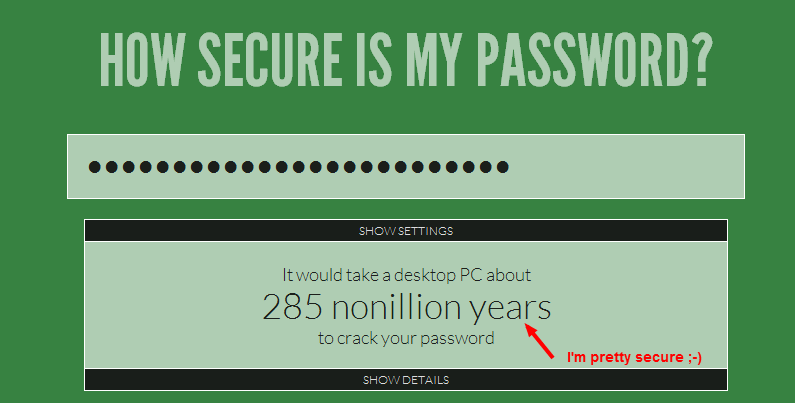
\includegraphics[scale=0.1]{pics/bruteforce2.png}
	\end{figure}

	\clearpage
	Nowadays, a common attacks are based on Rainbow Tables, a special type of lookup table used in 
	recovering the plaintext password from a ciphertext generated by a one-way hash.
	Tables are specific to the hash function they were created for e.g., MD5 tables can only crack MD5 
	hashes. The more powerful RainbowCrack program was later developed that can generate and use rainbow
	tables for a variety of character sets and hashing algorithms, including LM hash, MD5, SHA1, etc.

	\begin{figure}[H]
		
\includegraphics[width=\textwidth]{pics/rainbow.png}
	\end{figure}




\section{Bypassing Authentication Schema}

	While most applications require authentication for gaining access to private information or 
	to execute tasks, not every authentication method is able to provide adequate security.
	There are several methods to bypass the authentication schema in use by a web application:
		\begin{itemize}
			\item Direct page request (forced browsing)
			\item Parameter Modification
			\item Session ID Prediction
			\item SQL Injection
		\end{itemize}


\section{Vulnerable remember password and reset}
	Most web applications allow users to reset their password if they have forgotten it, usually 
	by sending them a password reset email and/or by asking them to answer one or more 
	"security questions".

	A great majority of web applications provide a way for users to recover (or reset) their password 
	in case they have forgotten it. The exact procedure varies heavily among different applications, 
	also depending on the required level of security, but the approach is always to use an alternate 
	way of verifying the identity of the user. One of the simplest (and most common) approaches is 
	to ask the user for his/her e-mail address, and send the old password (or a new one) to that
	address. This scheme is based on the assumption that the user's email has not been compromised 
	and that is secure enough for this goal.

	Alternatively (or in addition to that), the application could ask the user to answer one or more 
	"secret questions", which are usually chosen by the user among a set of possible ones. 
	The security of this scheme lies in the ability to provide a way for someone to identify themselves 
	to the system with answers to questions that are not easily answerable via personal information 
	lookups. As an example, a very insecure question would be “your mother’s maiden name” since that 
	is a piece of information that an attacker could find out without much effort. An example of a 
	better question would be “favorite grade-school teacher” since this would be a much more difficult 
	topic to research about a person whose identity may otherwise already be stolen.

	Another common feature that applications use to provide users a convenience, is to cache the 
	password locally in the browser (on the client machine) and having it 'pre-typed' in all 
	subsequent accesses. While this feature can be perceived as extremely friendly for the average 
	user, at the same time it introduces a flaw, as the user account becomes easily accessible
	to anyone that uses the same machine account.

\section{Browser Cache Management}
	In this phase, we check that the logout function is properly implemented, and that it is not 
	possible to “reuse” a session after logout. We also check that the application automatically 
	logs out a user when that user has been idle for a certain amount of time, and that no sensitive 
	data remains stored in the browser cache.

	{\bf Logout function:} \\
	The first step is to test the presence of the logout function. Check that the application provides 
	a logout button and that this button is present and well visible on all pages that require  
	authentication. A logout button that is not clearly visible, or that is present only on certain 
	pages, poses a security risk, as the user might forget to use it at the end of his/her session.
	The second step consists in checking what happens to the session tokens when the logout function 
	is invoked. For instance, when cookies are used a proper behavior is to erase all session cookies, 
	by issuing a new Set-Cookie directive that sets their value to a non-valid one (e.g.: “NULL” or 
	some equivalent value) and, if the cookie is persistent, setting its expiration date in the past, 
	which tells the browser to discard the cookie. The first (and simplest) test at this point consists 
	of logging out and then hitting the 'back' button of the browser, to check whether we are still
	authenticated. If we are, it means that the logout function has been implemented insecurely, and 
	that the logout function does not destroy the session IDs. It should be noted that this test only 
	applies to session cookies, and that a persistent cookie that only stores data about some minor 
	user preferences (e.g.: site appearance) and that is not deleted when the user logs out is not 
	to be considered a security risk.

	{\bf Timeout logout:} \\
	The most appropriate logout time should be a right balance between security (shorter logout time) 
	and usability (longer logout time) and heavily depends on the criticality of the data handled by 
	the application. A 60 minute logout time for a public forum can be acceptable, but such a long time 
	would be way too much in a home banking application.

	{\bf Cached pages:} \\
	Logging out from an application obviously does not clear the browser cache of any sensitive 
	information that might have been stored. Therefore, another test that is to be performed is to 
	check that our application does not leak any critical data into the browser cache. In order to 
	do that, we can use WebScarab and search through the server responses that belong to our session,
	checking that for every page that contains sensitive information the server instructed the browser 
	not to cache any data. Such a directive can be issued in the HTTP response headers. 

	{\bf As a general rule, we need to check that:}
		\begin{itemize}
			\item The logout function effectively destroys all session token, or at least renders 
			them unusable
			\item The server performs proper checks on the session state, disallowing an attacker 
			to replay some previous token.
			\item A timeout is enforced and it is properly checked by the server. If the server 
			uses an expiration time that is read from a session token that is sent by the client, 
			the token must be cryptographically protected.
		\end{itemize}

\section{Captcha}
	{\bf CAPTCHA ("Completely Automated Public Turing test to tell Computers and Humans Apart")} is a
	type of challenge-response test used by many web applications to ensure that the response is not
	generated by a computer. CAPTCHA implementations are often vulnerable to various kinds of attacks 
	even if the generated CAPTCHA is unbreakable. This section will help you to identify these kinds 
	of attacks.

	Although CAPTCHA is not an authentication control, its use can be very efficient against:
		\begin{itemize}
			\item enumeration attacks (login, registration or password reset forms are often vulnerable 
			to enumeration attacks - without CAPTCHA the attacker can gain valid usernames, phone numbers 
			or any other sensitive information in a short time)
			\item automated sending of many GET/POST requests in a short time where it is undesirable 
			(e.g., SMS/MMS/email flooding), CAPTCHA provides a rate limiting function
			\item automated creation/using of the account that should be used only by humans 
			(e.g., creating webmail accounts, stop spamming)
			\item automated posting to blogs, forums and wikis, whether as a result of commercial 
			promotion, or harassment and vandalism
			\item any automated attacks that massively gain or misuse sensitive information from 
			the application
		\end{itemize}

	These vulnerabilities are quite common in many CAPTCHA implementations:
	\begin{itemize}
		\item generated image CAPTCHA is weak, this can be identified (without any complex computer
		recognition systems) only by a simple comparison with already broken CAPTCHAs
		\item generated CAPTCHA questions have a very limited set of possible answers
		\item the value of decoded CAPTCHA is sent by the client (as a GET parameter or as a 
		hidden field of POST form). This value is often: {\bf 1)} encrypted by simple algorithm and 
		can be easily decrypted by observing of multiple decoded CAPTCHA values. 
		{\bf 2)} hashed by a weak hash function (e.g., MD5) that can be broken using a rainbow 
		table 
		\item possibility of replay attacks:
			{\bf 1)} the application does not keep track of what ID of CAPTCHA image is sent to 
			the user. Therefore, the attacker can simply obtain an appropriate CAPTCHA image and 
			its ID, solve it, and send the value of the decoded CAPTCHA with its corresponding ID 
			(the ID of a CAPTCHA could be a hash of the decoded CAPTCHA or any unique identifier)
			{\bf 2)} the application does not destroy the session when the correct phrase is entered 
			- by reusing the session ID of a known CAPTCHA it is possible to bypass CAPTCHA protected 
			page
	\end{itemize}


\section{Multiple Factors Authentication}

	“Multiple Factors Authentication System” (MFAS) is a critical task for the Penetration tester.
	Generally the aim of a two factor authentication system is to enhance the strength of the 
	authentication process. This goal is achieved by checking an additional factor, or “something 
	you have” as well as “something you know”, making sure that the user holds a hardware device of 
	some kind in addition to the password. The hardware device provided to the user may be able to
	communicate directly and independently with the authentication infrastructure using an additional
	communication channel; this particular feature is something known as “separation of channels”.
	Bruce Schneier in 2005 observed that some years ago “the threats were all passive: eavesdropping 
	and offline password guessing. Today, the threats are more active: phishing and Trojan horses”. 
	Actually the common threats that a MFAS in a Web environment should correctly address include:
		\begin{enumerate}
			\item Weak Credentials (Credentials Password guessing and Password Bruteforcing attacks)
			\item Credential Theft (Phishing, Eavesdropping, MITM e.g. Banking from compromised network)
			\item Session based attacks (Session Riding, Session Fixation)
			\item Trojan and Malware attacks (Banking from compromised clients)
			\item Password Reuse (Using the same password for different purposes or operations, 
			e.g. different transactions)
		\end{enumerate}

	The typical IT professional’s advise is: “If you are not happy with your current
	authentication solution, just add another authentication factor and it will be all right”.

	MFAS solutions add “something you have” to the authentication process. This component is usually a:
		\begin{itemize}
			\item One-time password (OTP) generator token.
			\item Grid Card, Scratch Card, or any information that only the legitimate user is 
			supposed to have in his wallet
			\item Crypto devices like USB tokens or smart cards.
			\item Randomly generated OTPs transmitted through a GSM SMS messages.
		\end{itemize}

\section{Race Conditions}

	A race condition is a flaw that produces an unexpected result when the timing of actions impact 
	other actions. An example may be seen on a multithreaded application where actions are being 
	performed on the same data. Race conditions, by their very nature, are difficult to test for.

	Race conditions may occur when a process is critically or unexpectedly dependent on the sequence 
	or timings of other events. In a web application environment, where multiple requests can be 
	processed at a given time, developers may leave concurrency to be handled by the framework, 
	server, or programming language. The following simplified example illustrates a potential 
	concurrency problem in a transactional web application and relates to a joint savings account 
	in which both users (threads) are logged into the same account and attempting a transfer.

	{\bf \color{red} Account A has 100 credits}

	{\bf \color{blue} Account B has 100 credits}

	Both User 1 and User 2 want to transfer 10 credits from Account A to Account B. If the 
	transaction was correct the outcome should be:

	{\bf \color{red} Account A has 80 credits}

	{\bf \color{blue} Account B has 120 credits}

	However, due to concurrency issues, the following result could be obtained:

	{\bf User 1 checks the value of Account A (=100 credits)}

	{\bf User 2 checks the value of Account A (=100 credits)}

	{\bf User 2 takes 10 credits from Account A (=90 credits) and put it in Account B (=110 credits)}

	{\bf User 1 takes 10 credits from Account A (Still believed to contain 100 credits) 
	(=90 credits) and puts it into Account B (=120 credits).}

	{\bf \color{red} Result: Account A has 90 credits}
	
	{\bf \color{blue} Account B has 120 credits}

	However, testing can be focused on specific transactional areas of the application, where 
	time-of-read to time-of-use of specific data variables could be adversely affected by concurrency 
	issues.



	\clearpage
	\chapter{Session Management Testing}

	At the core of any web-based application is the way in which it maintains state and thereby 
	controls user-interaction with the site. Session Management broadly covers all controls on 
	a user from  authentication to leaving the application. HTTP is a stateless protocol, meaning 
	that web servers respond to client requests without linking them to each other. Even simple
	application logic requires a user's multiple requests to be associated with each other across 
	a "session”. Most popular web application environments, such as ASP and PHP, provide developers 
	with built-in session handling routines. Some kind of identification token will typically be issued, 
	which will be referred to as a “Session ID” or Cookie.

	\begin{figure}[H]
		
\includegraphics[scale=0.4]{pics/cookie.jpg}
	\end{figure}

	\clearpage
	\section{Session Management Schema}

		This describes how to analyse a Session Management Schema, with the goal to understand how 
		the Session Management mechanism has been developed and if it is possible to break it to 
		bypass the user session. It explains how to test the security of session tokens issued to 
		the client's browser: how to reverse engineer a cookie, and how to manipulate cookies
		to hijack a session.

		In order to avoid continuous authentication for each page of a website or service, web applications implement various mechanisms to store and validate credentials for a pre-determined timespan.
		These mechanisms are known as Session Management and, while they're most important in order to increase the ease of use and user-friendliness of the application.

		Cookies are used to implement {\bf session management}. In a nutshell, when a user accesses an 
		application which needs to keep track of the actions and identity of that user across multiple
		requests, a cookie (or more than one) is generated by the server and sent to the client. 
		The client will then send the cookie back to the server in all following connections until 
		the cookie expires or is destroyed. The data stored in the cookie can provide to the server
		a large spectrum of information about who the user is, what actions he has performed so far, 
		what his preferences are, etc. therefore providing a state to a {stateless protocol like HTTP}.
		
		A typical example is provided by an {\bf online shopping cart}. Throughout the session of a user, 
		the application must keep track of his identity, his profile, the products that he has chosen to 
		buy, the quantity, the individual prices, the discounts, etc.
		Cookies are an efficient way to store and pass this information back and forth (other methods are 
		URL parameters and hidden fields).
		
		Due to the importance of the data that they store, cookies are therefore vital in the overall 
		security of the application. Being able to tamper with cookies may result in hijacking the 
		sessions of legitimate users, gaining higher privileges in an active session, and in general
		influencing the operations of the application in an unauthorized way. 

		Usually the main steps of the attack pattern are the following:
			\begin{itemize}
				\item {\bf Cookie collection:} collection of a sufficient number of cookie samples;
				\item {\bf Cookie reverse engineering:} analysis of the cookie generation algorithm;
				\item {\bf Cookie manipulation:} forging of a valid cookie in order to perform the 
				attack. This last step might require a large number of attempts, depending on how the 
				cookie is created (cookie brute-force attack).
				\item {\bf Cookie overflow:} Strictly speaking, this attack has a different nature. Instead 
				of getting a valid cookie, our goal is to overflow a memory area, thereby interfering
				with the correct behavior of the application and possibly injecting (and remotely 
				executing) malicious code.
			\end{itemize}

		\subsection{Cookie Collection and Session Analysis}

			The first step required in order to manipulate the cookie is obviously to understand how 
			the application creates and manages cookies. For this task, we have to try to answer the
			following questions: 

			{\bf How many cookies are used by the application?} \\
			Surf the application. Note when cookies are created. Make a list of received cookies, 
			the page that sets them (with the set-cookie directive), the domain for which they are 
			valid, their value, and their characteristics.

			{\bf Which parts of the application generate and/or modify the cookie?} \\
			Surfing the application, find which cookies remain constant and which get modified. 
			What events modify the cookie?

			{\bf Which parts of the application require this cookie in order to be accessed and utilized?} \\
			Find out which parts of the application need a cookie. Access a page, then try again without 
			the cookie, or with a modified value of it. Try to map which cookies are used where.
			A spreadsheet mapping each cookie to the corresponding application parts and the related 
			information can be a valuable output of this phase.

			The session tokens (Cookie, SessionID or Hidden Field) themselves should be examined to 
			ensure their quality from a security perspective. They should be tested against criteria 
			such as their randomness, uniqueness, resistance to statistical and cryptographic analysis 
			and information leakage.


		\subsection{Token structure and Information Leakage}
			The first stage is to examine the structure and content of a Session ID provided by 
			the application. A common mistake is to {\bf include specific data} in the Token instead 
			of issuing a generic value and referencing real data at the server side. 
			If the Session ID is {\bf clear-text}, the structure and pertinent data may be immediately
			obvious as the following: \\
			{\bf Clear-text:} {\color{blue} 192.168.100.1:owaspuser:password:15:58} \\
			{\bf Hybrid:} {\color{blue} owaspuser:192.168.100.1: a7656fafe94dae72b1e1487670148412}

			If part or the entire token appears to be encoded or hashed, it should be compared to 
			various techniques to check for obvious obfuscation. Having identified the type of 
			obfuscation, it may be possible to decode back to the original data.

				\begin{figure}[H]
					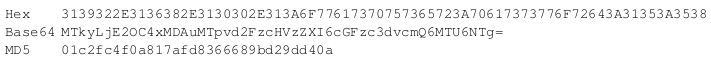
\includegraphics[width=\textwidth]{pics/cookies.png}
				\end{figure}

			A simple analysis of the tokens should immediately reveal any obvious patterns. 
			For example, a 32 bit token may include 16 bits of static data and 16 bits
			of variable data. This may indicate that the first 16 bits represent a fixed attribute 
			of the user – e.g. the username or IP address. If the second 16 bit chunk is incrementing 
			at a regular rate, it may indicate a sequential or even time-based element to the token
			generation.The following areas should be addressed during the single and multiple Session 
			ID structure testing:

				\begin{itemize}
					\item What parts of the Session ID are static?
					\item What clear-text confidential information is stored in the Session ID? 
					E.g. usernames/UID, IP addresses
					\item What easily decoded confidential information is stored?
					\item What information can be deduced from the structure of the Session ID?
					\item What portions of the Session ID are static for the same login conditions?
					\item What obvious patterns are present in the Session ID as a whole, or individual
					portions?
				\end{itemize}

		\subsection{Session ID Predictability and Randomness}
			Analysis of the variable areas (if any) of the Session ID should be undertaken to 
			establish the existence of any recognizable or predictable patterns. 
			In analyzing Session ID sequences, patterns or cycles, static elements and client 
			dependencies should all be considered as possible contributing elements to the structure 
			and function of the application:
				\begin{itemize}
					\item Are the Session IDs provably random in nature?
					\item Do the same input conditions produce the same ID on a subsequent run?
					\item Are the Session IDs provably resistant to statistical or cryptanalysis?
					\item What elements of the Session IDs are time-linked?
					\item What portions of the Session IDs are predictable?
					\item Can the next ID be deduced, given full knowledge of the generation algorithm 
					and previous IDs
				\end{itemize}

		\subsection{Cookie Reverse Engineering}
			Now that we have enumerated the cookies and have a general idea of their use, it is time to 
			have a deeper look at cookies that seem interesting. Which cookies are we interested in? 
			A cookie, in order to provide a secure method of session management, must combine several
			characteristics, each of which is aimed at protecting the cookie from a different class 
			of attacks. These characteristics are summarized below:

				\begin{enumerate}
					\item {\bf Unpredictability:} a cookie must contain some amount of hard-to-guess 
					data. The harder it is to forge a valid cookie, the harder is to break into 
					legitimate user's session. If an attacker can guess the cookie used in an active 
					session of a legitimate user, he/she will be able to fully impersonate that user 
					(session hijacking). In order to make a cookie unpredictable, random values 
					and/or cryptography can be used.
					\item {\bf Tamper resistance:} a cookie must resist malicious attempts of 
					modification. If we receive a cookie like IsAdmin=No,  it is trivial to modify it 
					to get administrative rights, unless the application performs a double check 
					(for instance, appending to the cookie an encrypted hash of its value)
					\item {\bf Expiration:} a critical cookie must be valid only for an appropriate 
					period of time and must be deleted from disk/memory afterwards, in order to avoid 
					the risk of being replayed. This does not apply to cookies that store non-critical 
					data that needs to be remembered across sessions (e.g., site look-and-feel)
					\item {\bf “Secure” flag:} a cookie whose value is critical for the integrity of 
					the session should have this flag enabled in order to allow its transmission only 
					in an encrypted channel to deter eavesdropping.
				\end{enumerate}

				\begin{figure}[H]
					\centering
					
\includegraphics[scale=0.5]{pics/deleteCookies.jpg}
				\end{figure}

			The approach here is to {\bf collect a sufficient number of instances of a cookie} and 
			start looking for {\bf patterns} in their value. The exact meaning of “sufficient” can vary 
			from a handful of samples, if the cookie generation method is very easy to break, to
			several thousands, if we need to proceed with some mathematical analysis.

			It is important to pay particular attention to the {\bf workflow of the application}, 
			as the state of a session can have a heavy impact on collected cookies: a cookie 
			collected before being authenticated can be very different from a cookie obtained
			after the authentication.

			Another aspect to keep into consideration is {\bf time}: always record the exact time 
			when a cookie has been obtained, when there is the possibility that time plays a role 
			in the value of the cookie (the server could use a timestamp as part of the
			cookie value).

			{\bf Analyzing the collected values}, try to figure out all variables that could have 
			influenced  the cookie value and try to vary them one at the time. Passing to the server 
			modified versions of the same cookie can be very helpful in understanding how the 
			application reads and processes the cookie.

		\subsection{Brute Force Attacks}
			Brute force attacks inevitably lead on from questions relating to predictability and 
			randomness. The variance within the Session IDs must be considered together with 
			application session durations and timeouts. If the variation within the Session
			IDs is relatively small, and Session ID validity is long, the likelihood of a successful 
			brute-force attack is much higher. A long Session ID (or rather one with a great deal 
			of variance) and a shorter validity period would make it far harder to succeed in a
			brute force attack.

		\clearpage
		\subsection{Cookie Manipulation}
			Once you have squeezed out as much information as possible from the cookie, it is 
			time to start to modify it. The methodologies here heavily depend on the results 
			of the analysis phase, but we can provide some examples:

			{\bf Example 1: Guessable Cookie} \\
			An example of a cookie whose value is easy to guess and that can be used to impersonate 
			other users can be found in OWASP WebGoat, in the “Weak Authentication cookie” lesson. 
			In this example, you start with the knowledge of two username/password couples 
			(corresponding to the users 'webgoat' and 'aspect'). The goal is to reverse engineer 
			the cookie creation logic and break into the account of user 'alice'. 
			Authenticating to the application using these known couples, you can collect the 
			corresponding authentication cookies.

			\begin{figure}[H]
				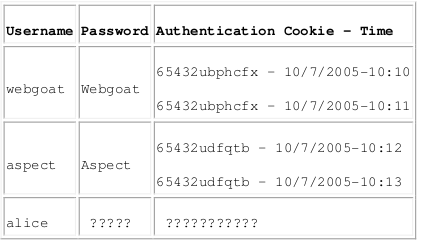
\includegraphics[scale=0.5]{pics/exampleCookie.png}
			\end{figure}

			First of all, we can note that the authentication cookie remains constant for the same 
			user across different logons, showing a first critical vulnerability to replay attacks: 
			if we are able to steal a valid cookie (using for example a XSS vulnerability), we
			can use it to hijack the session of the corresponding user without knowing his/her 
			credentials. Additionally, we note that the “webgoat” and “aspect” cookies have a 
			common part: “65432u”. So let's see the letter following each letter in “webgoat”:

			\begin{figure}[H]
				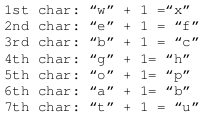
\includegraphics[scale=0.5]{pics/webgoat.png}
			\end{figure}

			We obtain “xfchpbu”, which inverted gives us exactly “ubphcfx”. The algorithm fits 
			perfectly also for the user 'aspect', so we only have to apply it to user 'alice'.
			Bingo! Now can the application identifies us as “alice” instead of “webgoat”.

		\subsection{Brute Force}

		The use of a brute force attack to find the right authentication cookie, could be a 
		heavy time consuming technique. Foundstone Cookie Digger can help to collect a large 
		number of cookies, giving the average length and the character set of the cookie. 
		In advance, the tool compares the different values of the cookie to check how many 
		characters are changing for every subsequent login. If the cookie values do not 
		remain the same on subsequent logins, Cookie Digger gives the attacker longer periods 
		of time to perform brute force attempts. In the following table we show an example 
		in which we have collected all the cookies from a public site, trying 10 authentication 
		attempts. For every type of cookie collected you have an estimate of all the possible 
		attempts needed to “brute force” the cookie.

		\begin{figure}[H]
			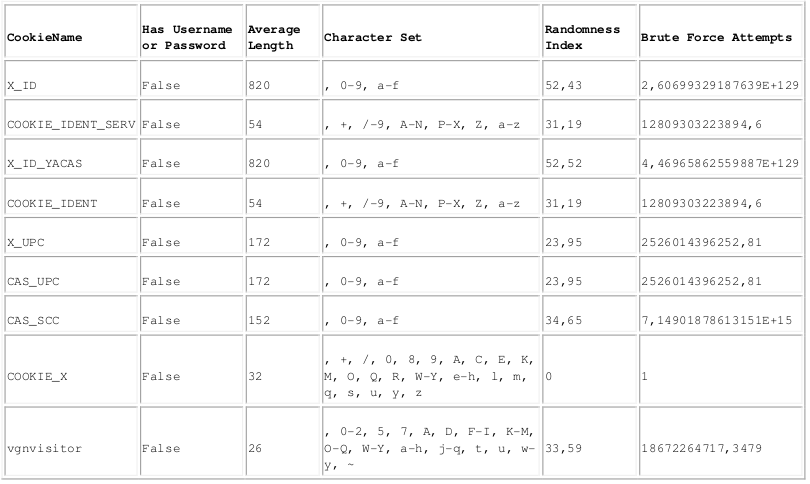
\includegraphics[width=\textwidth]{pics/bruteforce.png}
		\end{figure}

		\subsection{Overflow}
			Since the cookie value, when received by the server, will be stored in one or more 
			variables, there is always the chance of performing a boundary violation of that 
			variable. Overflowing a cookie can lead to all the outcomes of buffer overflow
			attacks. A Denial of Service is usually the easiest goal, but the execution of 
			remote code can also be possible. Usually, however, this requires some detailed 
			knowledge about the architecture of the remote system, as any buffer overflow
			technique is heavily dependent on the underlying operating system and memory 
			management in order to correctly calculate offsets to properly craft and align 
			inserted code.

	\section{Cookies Attributes}

		Cookies are often a key attack vector for malicious users (typically targeting other users) 
		and, as such, the application should always take due diligence to protect cookies. In this 
		section, we will look at how an application can take the necessary precautions when assigning 
		cookies and how to test that these attributes have been correctly configured.

		As you can imagine, there are many different types of applications that need to keep track 
		of session state across multiple requests. The primary one that comes to mind would be an 
		online store. As a user adds multiple items to a shopping cart, this data needs to be retained 
		in subsequent requests to the application. Cookies are very commonly used for this task and 
		are set by the application using the Set-Cookie directive in the application's HTTP response, 
		and is usually in a name=value format. Once an application has told the browser to use a 
		particular cookie, the browser will send this cookie in each subsequent request. 
		A cookie can contain data such as items from an online shopping cart, the price of these items, 
		the quantity of these items, personal information, user IDs, etc. D
		ue to the sensitive nature of information in cookies, they are typically encoded or encrypted 
		in an attempt to protect the information they contain. 

		Let's take a look at what attributes can be set for a cookie. 
		The following is a list of the attributes that can be set for each cookie and 
		what they mean:

		\begin{itemize}
			\item {\bf Secure} - This attribute tells the browser to only send the cookie if the 
			request is being sent over a secure channel such as HTTPS. If the application can be 
			accessed over both HTTP and HTTPS, then there is the potential that the cookie can be 
			sent in clear text.
			\item {\bf HttpOnly} - This attribute is used to help prevent attacks such as cross-site
			scripting, since it does not allow the cookie to be accessed via a client side script 
			such as JavaScript. 
			\item {\bf Domain} - This attribute is used to compare against the domain of the server 
			in which the URL is being requested. 
			\item {\bf Path} - In addition to the domain, the URL path can be specified for which 
			the cookie is valid. If the domain and path match, then the cookie will be sent in the 
			request.
			\item {\bf Expires} - This attribute is used to set persistent cookies, since the cookie 
			does not expire until the set date is exceeded. This persistent cookie will be used by 
			this browser session and subsequent sessions until the cookie expires. Once the expiration 
			date has exceeded, the browser will delete the cookie.
		\end{itemize}

	\section{Session Fixation}

	\section{Exposed Session Variables}

	\section{CSRF}

		CSRF is an attack which forces an end user to execute unwanted actions on a web application 
		in which he/she is currently authenticated. With a little help of {\bf social engineering} 
		(like sending a link via email/chat), an attacker may force the users of a web application 
		to execute actions of the attacker's choosing. A successful CSRF exploit can compromise end 
		user data and operation, when it targets a normal user. 
	\clearpage
	\chapter{Authorization Testing}
	\clearpage
	\chapter{Business Logic Testing}

	Testing for business logic flaws in a multi-functional dynamic web application requires thinking 
	in unconventional ways. This type of vulnerability cannot be detected by a vulnerability scanner 
	and relies upon the skills and creativity of the penetration tester. In addition, this type of
	vulnerability is usually one of the hardest to detect, but, at the same time, usually one of the 
	most detrimental to the application, if exploited. Attacks on the business logic of an application 
	are dangerous, difficult to detect, and are usually specific to the application being tested.

	{\bf Business logic may include:}
	\begin{itemize}
		\item {\bf Business rules} that express business policy (such as channels, location, logistics, 
		prices, and products);
		\item  {\bf Workflows} based on the ordered tasks of passing documents or data from one participant 
		(a person or a software system) to another. 
	\end{itemize}


	Business logic can have security flaws that allow a user to do something that isn't allowed by the
	business. For example, if there is a limit on reimbursement of \$1000, could an attacker misuse the 
	system to request more money than it is intended? Or, perhaps, users are supposed to do operations 
	in a particular order, but an attacker could invoke them out of sequence. Or can a user make a 
	purchase for a negative amount of money?

	{\bf Example 1:}\\
	Setting the quantity of a product on an e-commerce site as a negative number may result in funds 
	being credited to the attacker. The countermeasure to this problem is to implement stronger data
	validation, as the application permits negative numbers to be entered in the quantity field of 
	the shopping cart.

	{\bf Example 2:} \\
	Another more complex example pertains to a commercial financial application that a large institution 
	uses for their business customers. When a user is created by an administrator account, a new userid 
	is associated with this new account. The userids that are created are predictable. For example, 
	if an admin from a fictitious customer of "Spacely Sprockets" creates two accounts consecutively, 
	their respective userids will be 115 and 116. To make things worse, if two more accounts are created 
	and their respective userids are 117 and 119, then it can be assumed that another company's admin 
	has created a user account for their company with the userid of 118.

	{\bf Creating Raw Data for Designing Logical Tests} \\
		\begin{itemize}
			\item {\bf All application business scenarios:} Checkout, Browse, Product ordering, Search for a 
			product, etc.
			\item {\bf Workflows}
			\item {\bf Different user roles:} Manager, Staff, Administrator, CEO, etc.
			\item {\bf Different groups or departments:} Purchasing, Marketing, Engineering, etc.
			\item {\bf Access Rights of Various User Roles and Groups}
			\item {\bf Privilege Table}
		\end{itemize}



	\clearpage
	\chapter{Data Validation Testing}

	The most common web application security weakness is the failure to properly validate input coming 
	from the client or environment before using it.  Data validation is the task of testing all the 
	possible forms of input, to understand if the application sufficiently validates input data before 
	using it.

\section{Cross Site Scripting (XSS)}

	In Cross Site Scripting (XSS) testing, we test if it is possible to manipulate the input parameters 
	of the application so that it generates malicious output. We find an XSS vulnerability when the
	application does not validate our input and creates an output that is under our control. 

	\subsection{Refelcted Cross Site Scripting}
		Reflected XSS attacks are also known as {\bf type 1 or non-persistent XSS} attacks, and are 
		the most frequent type of XSS attacks found nowadays.
		When a web application is vulnerable to this type of attack, it will pass unvalidated input 
		sent through requests to the client. The common modus operandi of the attack includes a design 
		step, in which the attacker creates and tests an offending URI, a social engineering step, 
		in which she convinces her victims to load this URI on their browsers, and the eventual execution 
		of the offending code — using the victim's credentials.

		One of the important matters about exploiting XSS vulnerabilities is {\bf character encoding}. 
		In some cases, the web server or the web application could not be filtering some encodings of
		characters, so, for example, the web application might filter out a script tag, but might not 
		filter \%3cscript\%3e which simply includes another encoding of tags. 

		{\bf Example:}

		consider a site that has a welcome notice " Welcome \%username\% " and a download link.


		\begin{figure}[H]
			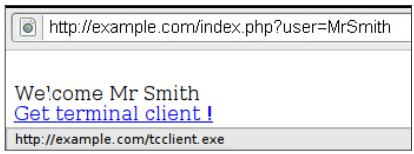
\includegraphics[scale=0.5]{pics/xxs1.png}
		\end{figure}

		To analyze it, the tester will play with the user variable and try to trigger the vulnerability. 
		Let's try to click on the following link and see what happens: 

		\begin{figure}[H]
			
\includegraphics[scale=0.5]{pics/link.png}
		\end{figure}
		If no sanitization is applied this will result in the following popup:

		\begin{figure}[H]
			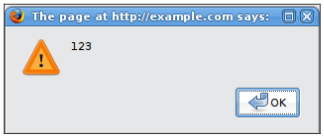
\includegraphics[scale=0.5]{pics/xss2.png}
		\end{figure}

		This indicates that there is an XSS vulnerability and it appears that the tester can execute 
		code of his choice in anybody's browser if he clicks on the tester's link.

	\clearpage
	\subsection{Stored Cross Site Scripting}

		Stored Cross Site Scripting (XSS) is the most dangerous type of Cross Site Scripting. 
		Web applications that allow users to store data are potentially exposed to this type of 
		attack. Stored XSS occurs when a web application gathers input from a user which might 
		be malicious, and then stores that input in a data store for later use. The input that 
		is stored is not correctly filtered. As a consequence, the malicious data will appear
		to be part of the web site and run within the user’s browser under the privileges of the 
		web application. Stored XSS does not need a malicious link to be exploited. 
		A successful exploitation occurs when a user visits a page with a stored XSS.

		The first step is to identify all points where user input is stored into the back-end and 
		then displayed by the application. Typical examples of stored user input can be found in:
		User/Profiles page, shopping cart, file managers, application settings/preferences, etc.

		{\bf Example: }

		\begin{figure}[H]
			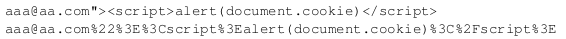
\includegraphics[scale=0.5]{pics/link2.png}
		\end{figure}
		\begin{figure}[H]
			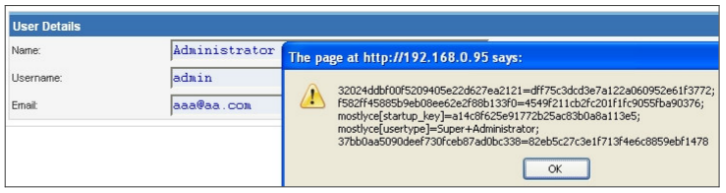
\includegraphics[scale=0.5]{pics/xss3.png}
		\end{figure}

	\subsection{DOM based Cross Site Scripting}
		Not all XSS bugs require the attacker to control the content returned from the server, but 
		can rather abuse poor JavaScript coding practices to achieve the same results. 
		The results are the same as a typical XSS bug, only the means of delivery is different.
		In comparison to other cross site scripting vulnerabilities (reflected and stored XSS), 
		where an unsanitized parameter is passed by the server, returned to the user and executed 
		in the context of the user’s browser, a DOM based cross site scripting vulnerability controls 
		the flow of the code by using elements of the Document Object Model (DOM) along with code 
		crafted by the attacker to change the flow.

		An attacker may append \# \textless script\textgreater alert('xss')\textless /script\textgreater to the affected page URL which would, 
		when executed display the alert box. In this instance, the appended code would not be sent 
		to the server as everything after the \# character is not treated as part of the query by 
		the browser but yet as a fragment. In this example the code is immediately executed and an
		alert of "xss" is displayed in the page. Unlike the more common types of cross site scripting 
		(persistent and non-persistent), in which the code is sent to the server and redisplayed to 
		the user, this is immediately executed in the user’s browser.


	\subsection{Cross Site Flashing}
	**RELEVANT?**

\section{SQL Injections (SQLi)}
	A SQL injection attack consists of insertion or "injection" of a SQL query via the input data 
	from the client to the application. A successful SQL injection exploit can read sensitive data 
	from the database, modify database data (Insert/Update/Delete), execute administration operations 
	on the database (such as shutdown the DBMS), recover the content of a given file existing on 
	the DBMS file system and, in some cases, issue commands to the operating system. 

	SQL Injection attacks can be divided into the following three classes:
		\begin{itemize}
			\item {\bf Inband:} data is extracted using the same channel that is used to inject the 
			SQL code. This is the most straightforward kind of attack, in which the retrieved data 
			is presented directly in the application web page.
			\item {\bf Out-of-band:} data is retrieved using a different channel (e.g., an email with the 
			results of the query is generated and sent to the tester).
			\item {\bf Inferential:} there is no actual transfer of data, but the tester is able to
			reconstruct the information by sending particular requests and observing the resulting 
			behaviour of the DB Server.
			\item {\bf Blind: } if the application hides the error details, then the tester must be 
			able to reverse engineer the logic of the original query.
		\end{itemize}

	{\bf SQL Injection Detection} \\
	The first step in this test is to understand when our application connects to a DB Server in order 
	to access some data. Typical examples of cases when an application needs to talk to a DB include:
	Authentication forms, search engines, E-Commerce sites, etc.

	The very first test usually consists of adding a single {\bf quote (')} or a {\bf semicolon (;)} 
	to the field  under test. The first is used in SQL as a string terminator and, if not filtered by 
	the application, would lead to an incorrect query. The second is used to end a SQL statement and, 
	if it is not filtered, it is also likely to generate an error. 

	{\bf Union Query SQL Injection} \\
	Another test involves the use of the UNION operator. This operator is used in SQL injections to 
	join a query, purposely forged by the tester, to the original query. The result of the forged 
	query will be joined to the result of the original query, allowing the tester to obtain the 
	values of fields of other tables.

	{\bf Blind SQL Injection} \\
	We have pointed out that there is another category of SQL injection, called Blind SQL Injection, 
	in which nothing is known on the outcome of an operation. For example, this behavior happens in 
	cases where the programmer has created a custom error page that does not reveal anything on 
	the structure of the query or on the database. (The page does not return a SQL error, it may 
	just return a HTTP 500).

	{\bf Stored Procedure Injections}
	When using dynamic SQL within a stored procedure, the application must properly sanitize the user 
	input to eliminate the risk of code injection. If not sanitized, the user could enter malicious 
	SQL that will be executed within the stored procedure.


\section{XML Injection}
	We talk about XML Injection testing when we try to inject an XML doc to the application: if the 
	XML parser fails to make an appropriate data validation the test will results positive.
	After lookking at a application, the tester will have some information about XML structure, 
	so it will be possible to try to inject XML data and tags (Tag Injection).

	{\bf Discovery} \\
	The first step in order to test an application for the presence of a XML Injection vulnerability,
	consists of trying to insert XML metacharacters.
	A list of some XML metacharacters is:
	\begin{itemize}
		\item Single quote {\bf '}
		\item Double quote {\bf "}
		\item Angular pharenthesis {\bf < >}
		\item Comment tag {\bf <!-- / -->}
		\item Ampersand {\bf \&}
	\end{itemize}

\section{SSI Injection}
	Web servers usually give to the developer the possibility of adding small pieces of dynamic code 
	inside static HTML pages, without having to play with full-fledged server-side or client-side 
	languages. This feature is incarnated by the Server-Side Includes (SSI), a very simple extension 
	that can enable an attacker to inject code into HTML pages, or even perform remote
	code execution.

	Putting an SSI directive into a static HTML document is as easy as writing a piece of code like 
	to print out the current time or like to include the content of a file.
	We could guess if SSI are supported just looking at the content of the target web site we are testing: 
	if it makes use of {\bf .shtml} files then SSI are probably supported, as this extension is used to
	identify pages containing these directives.

\section{Buffer Overflow}

	\subsection{Heap Overflow}
		Heap is a memory segment that is used for storing dynamically allocated data and global 
		variables. Each chunk of memory in heap consists of boundary tags that contain memory 
		management information. When a heap-based buffer is overflown, the control information 
		in these tags is overwritten, and when the heap management routine frees the buffer, 
		a memory address overwrite take place leading to an access violation. 

	\subsection{Stack Overflow}
		Stack overflows occur when variable size data is copied into fixed length buffers located 
		on the program stack without any bounds checking. 
		The key to testing an application for stack overflow vulnerabilities is supplying overly 
		large input data as compared to what is expected. 

	\clearpage
	\chapter{Denial of Service Testing}

	
	\clearpage
	\chapter{Web Services Testing}

	{\bf SOA (Service Orientated Architecture)/Web services applications} are up-and-coming systems 
	which are enabling businesses to interoperate and are growing at an unprecedented rate. 
	Webservice "clients" are generally not user web front-ends but other backend servers. 
	Webservices are exposed to the net like any other service but can be used on HTTP, FTP, SMTP, MQ
	among other transport protocols. The Web Services Framework utilizes the HTTP protocol 
	(as standard Web Application) in conjunction with XML, SOAP, WSDL and UDDI technologies:
		\begin{itemize}
			\item {\bf The "Web Services Description Language" (WSDL)} is used to describe the interfaces 
			of a service.
			\item {The "Simple Object Access Protocol" (SOAP)} provides the means for communication between 
			Web Services and Client Applications with XML and HTTP.
			\item {\bf "Universal Description, Discovery and Integration" (UDDI)} is used to register and
			publish Web Services and their characteristics so that they can be found from potential 
			clients.
		\end{itemize}

	The vulnerabilities in web services are similar to other vulnerabilities, such as SQL injection,
	information disclosure, and leakage, but web services also have unique XML/parser related 
	vulnerabilities, 

	\section{WS Information Gathering}
	{\bf Zero Knowledge} \\
	Normally you will have a WSDL path to access the Web Service, but if you have zero knowledge about it, 
	you will have to use UDDI to find a specific service. 

	{\bf WSDL endpoints} \\
	When a tester accesses the WSDL, he can determine an access point and available interfaces for web
	services. These interfaces or methods take inputs using SOAP over HTTP/HTTPS. If these inputs are 
	not defined well at the source code level, they can be compromised and exploited. 

	\section{HTTP GET Parameters/REST Testing}

		Many XML applications are invoked by passing them parameters using HTTP GET queries. 
		These are sometimes known as “REST-style" Web Services 
		{\bf (REST = Representational State Transfer)}. These Web Services can be attacked by 
		passing malicious content on the HTTP GET string. 

	\section{Replay Testing}

		This section describes testing replay vulnerabilities of a web service. The threat for a replay 
		attack is that the attacker can assume the identity of a valid user and commit some nefarious act
		without detection. A replay attack is a "man-in-the-middle" type of attack where a message is 
		intercepted and replayed by an attacker to impersonate the original sender. For web services, as 
		with other types of HTTP traffic, a sniffer such as Ethereal or Wireshark can capture traffic 
		posted to a web service and using a tool like WebScarab, a tester can resend a packet to the
		target server. An attacker can attempt to resend the original message or change the message in 
		order to compromise the host server.

{\color{red} **NOT FINISHED. IS THE CHAPTER VERY RELEVANT?**}




	\clearpage
	\chapter{AJAX Testing}
\end{document}
